%%%%%%%%%%%%%%%%%%%%%%%%%%%%%%%%%%%%%%%%%%%%%%%%%%%%%%%%%%%%%%%%%%%%%%%%%%%%%%%%
% AMS Beamer series / Bologna FC / Template
% Andrea Omicini
% Alma Mater Studiorum - Università di Bologna
% mailto:andrea.omicini@unibo.it
%%%%%%%%%%%%%%%%%%%%%%%%%%%%%%%%%%%%%%%%%%%%%%%%%%%%%%%%%%%%%%%%%%%%%%%%%%%%%%%%
%\documentclass[handout]{beamer}\mode<handout>{\usetheme{default}}
%
\documentclass[presentation, 10pt,aspectratio=169]{beamer}\mode<presentation>{\usetheme{AMSBolognaFC}}
%\documentclass[handout]{beamer}\mode<handout>{\usetheme{AMSBolognaFC}}
%%%%%%%%%%%%%%%%%%%%%%%%%%%%%%%%%%%%%%%%%%%%%%%%%%%%%%%%%%%%%%%%%%%%%%%%%%%%%%%%
\usetheme{metropolis}
  
\usepackage{lmodern}
\usepackage{fontawesome}
\usepackage[sfdefault]{FiraSans} %% option 'sfdefault' activates Fira Sans as the default text font
\usepackage[T1]{fontenc}
\renewcommand*\oldstylenums[1]{{\firaoldstyle #1}}
\usepackage{arev}
\usepackage{multicol}
\usepackage{wasysym}
\usepackage{amsmath,blkarray}
\usepackage{centernot}
\usepackage{fontawesome}
\usepackage{fancyvrb}
\usepackage[ddmmyyyy]{datetime}
\renewcommand{\dateseparator}{}
%\renewcommand{\thefootnote}{\fnsymbol{footnote}}
\newcommand{\version}{1}
\usepackage{biblatex}
	\makeatletter

% #FAFAFA
\definecolor{customfg}{RGB}{250, 250, 250} % White
% #23373B
\definecolor{custombg}{RGB}{35, 55, 59} % Dark Blue
\addbibresource{biblio.bib}
%%%%%%%%%%%%%%%%%%%%%%%%%%%%%%%%%%%%%%%%%%%%%%%%%%%%%%%%%%%%%%%%%%%%%%%%%%%%%%%%
\title[Il Potenziale dell'Intelligenza Artificiale Collettiva]
{Oltre l'IA Individuale: }
%
\subtitle[Il Potenziale dell'Intelligenza Artificiale Collettiva]
{Il Potenziale dell'Intelligenza Artificiale Collettiva}
%
\author[Aguzzi]
{\textbf{Gianluca Aguzzi} \href{mailto:gianluca.aguzzi@unibo.it}{gianluca.aguzzi@unibo.it}}
%
\institute[DISI, Univ.\ Bologna]
{Dipartimento di Informatica -- Scienza e Ingegneria (DISI)\\\textsc{Alma Mater Studiorum} -- Universit{\`a} di Bologna}
%
\renewcommand{\dateseparator}{/}
\date[\today]{\today}
%
%%%%%%%%%%%%%%%%%%%%%%%%%%%%%%%%%%%%%%%%%%%%%%%%%%%%%%%%%%%%%%%%%%%%%%%%%%%%%%%%ù
\metroset{block=fill}
\begin{document}

\nocite{*}
\frame{\titlepage}

{
\setbeamercolor{background canvas}{bg=custombg} % Set background to foreground color
\setbeamercolor{normal text}{fg=customfg}    

\begin{frame}[c]
	
	{
	\color{customfg}
	\begin{center}
	\Large\textbf{Hello World! :)}

	\begin{tikzpicture}
		\clip (0,0) circle (1.5cm) node {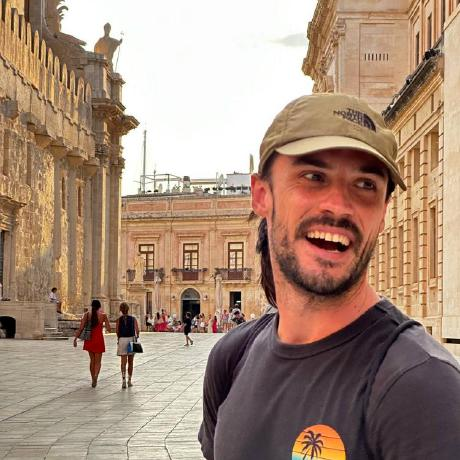
\includegraphics[width=3cm]{img/me-3.jpeg}};
	\end{tikzpicture}
	\color{customfg}{
	\small
	\begin{itemize}
		\color{customfg}
				\item \alert{\faGraduationCap} ~ \textbf{Dottorato} in Ingegneria e Scienze Informatiche (2024)
				\item \alert{\faPencilSquare} ~ \textbf{Professore a contratto} @ Università di Bologna (campus di Cesena)
				\item \alert{\faFlask} ~ \textbf{Background}: Ingegneria del Software (Sviluppatore Scala) \& Apprendimento Automatico (Apprendimento per Rinforzo)
				\item \alert{\faSearch} ~ \textbf{Interessi di Ricerca}: Intelligenza Collettiva, Apprendimento per Rinforzo Multi-Agente
			\end{itemize}
	}
	\end{center}
}
\end{frame}
}

\begin{frame}{Outline}
	\begin{itemize}
		\item Oggi parleremo di \alert{\textbf{Intelligenza Collettiva}} e \alert{\textbf{Sistemi Collettivi Adattativi}}, focalizzandosi su
		\begin{itemize}
			\item Cosa sono e come si differenziano da altri sistemi
			\item Come si progettano sistemi che mostrano intelligenza collettiva
			\begin{itemize}
				\item \emph{Approcci manuali} (ispirati biologia, programmazione aggregata)
				\item \emph{Approcci automatici} (algoritmi genetici, apprendimento per rinforzo multi-agente)
			\end{itemize}
			\item Direzioni di ricerca
			\begin{itemize}
				\item \emph{Approcci ibridi}
				\item Modelli fondazionali per l'intelligenza collettiva
			\end{itemize}
			Ma prima, un po' di contesto... :)
		\end{itemize}
	\end{itemize}
\end{frame}

\section{Contesto - Sistemi Collettivi Adattativi}
%% change the background image
{
\usebackgroundtemplate%
{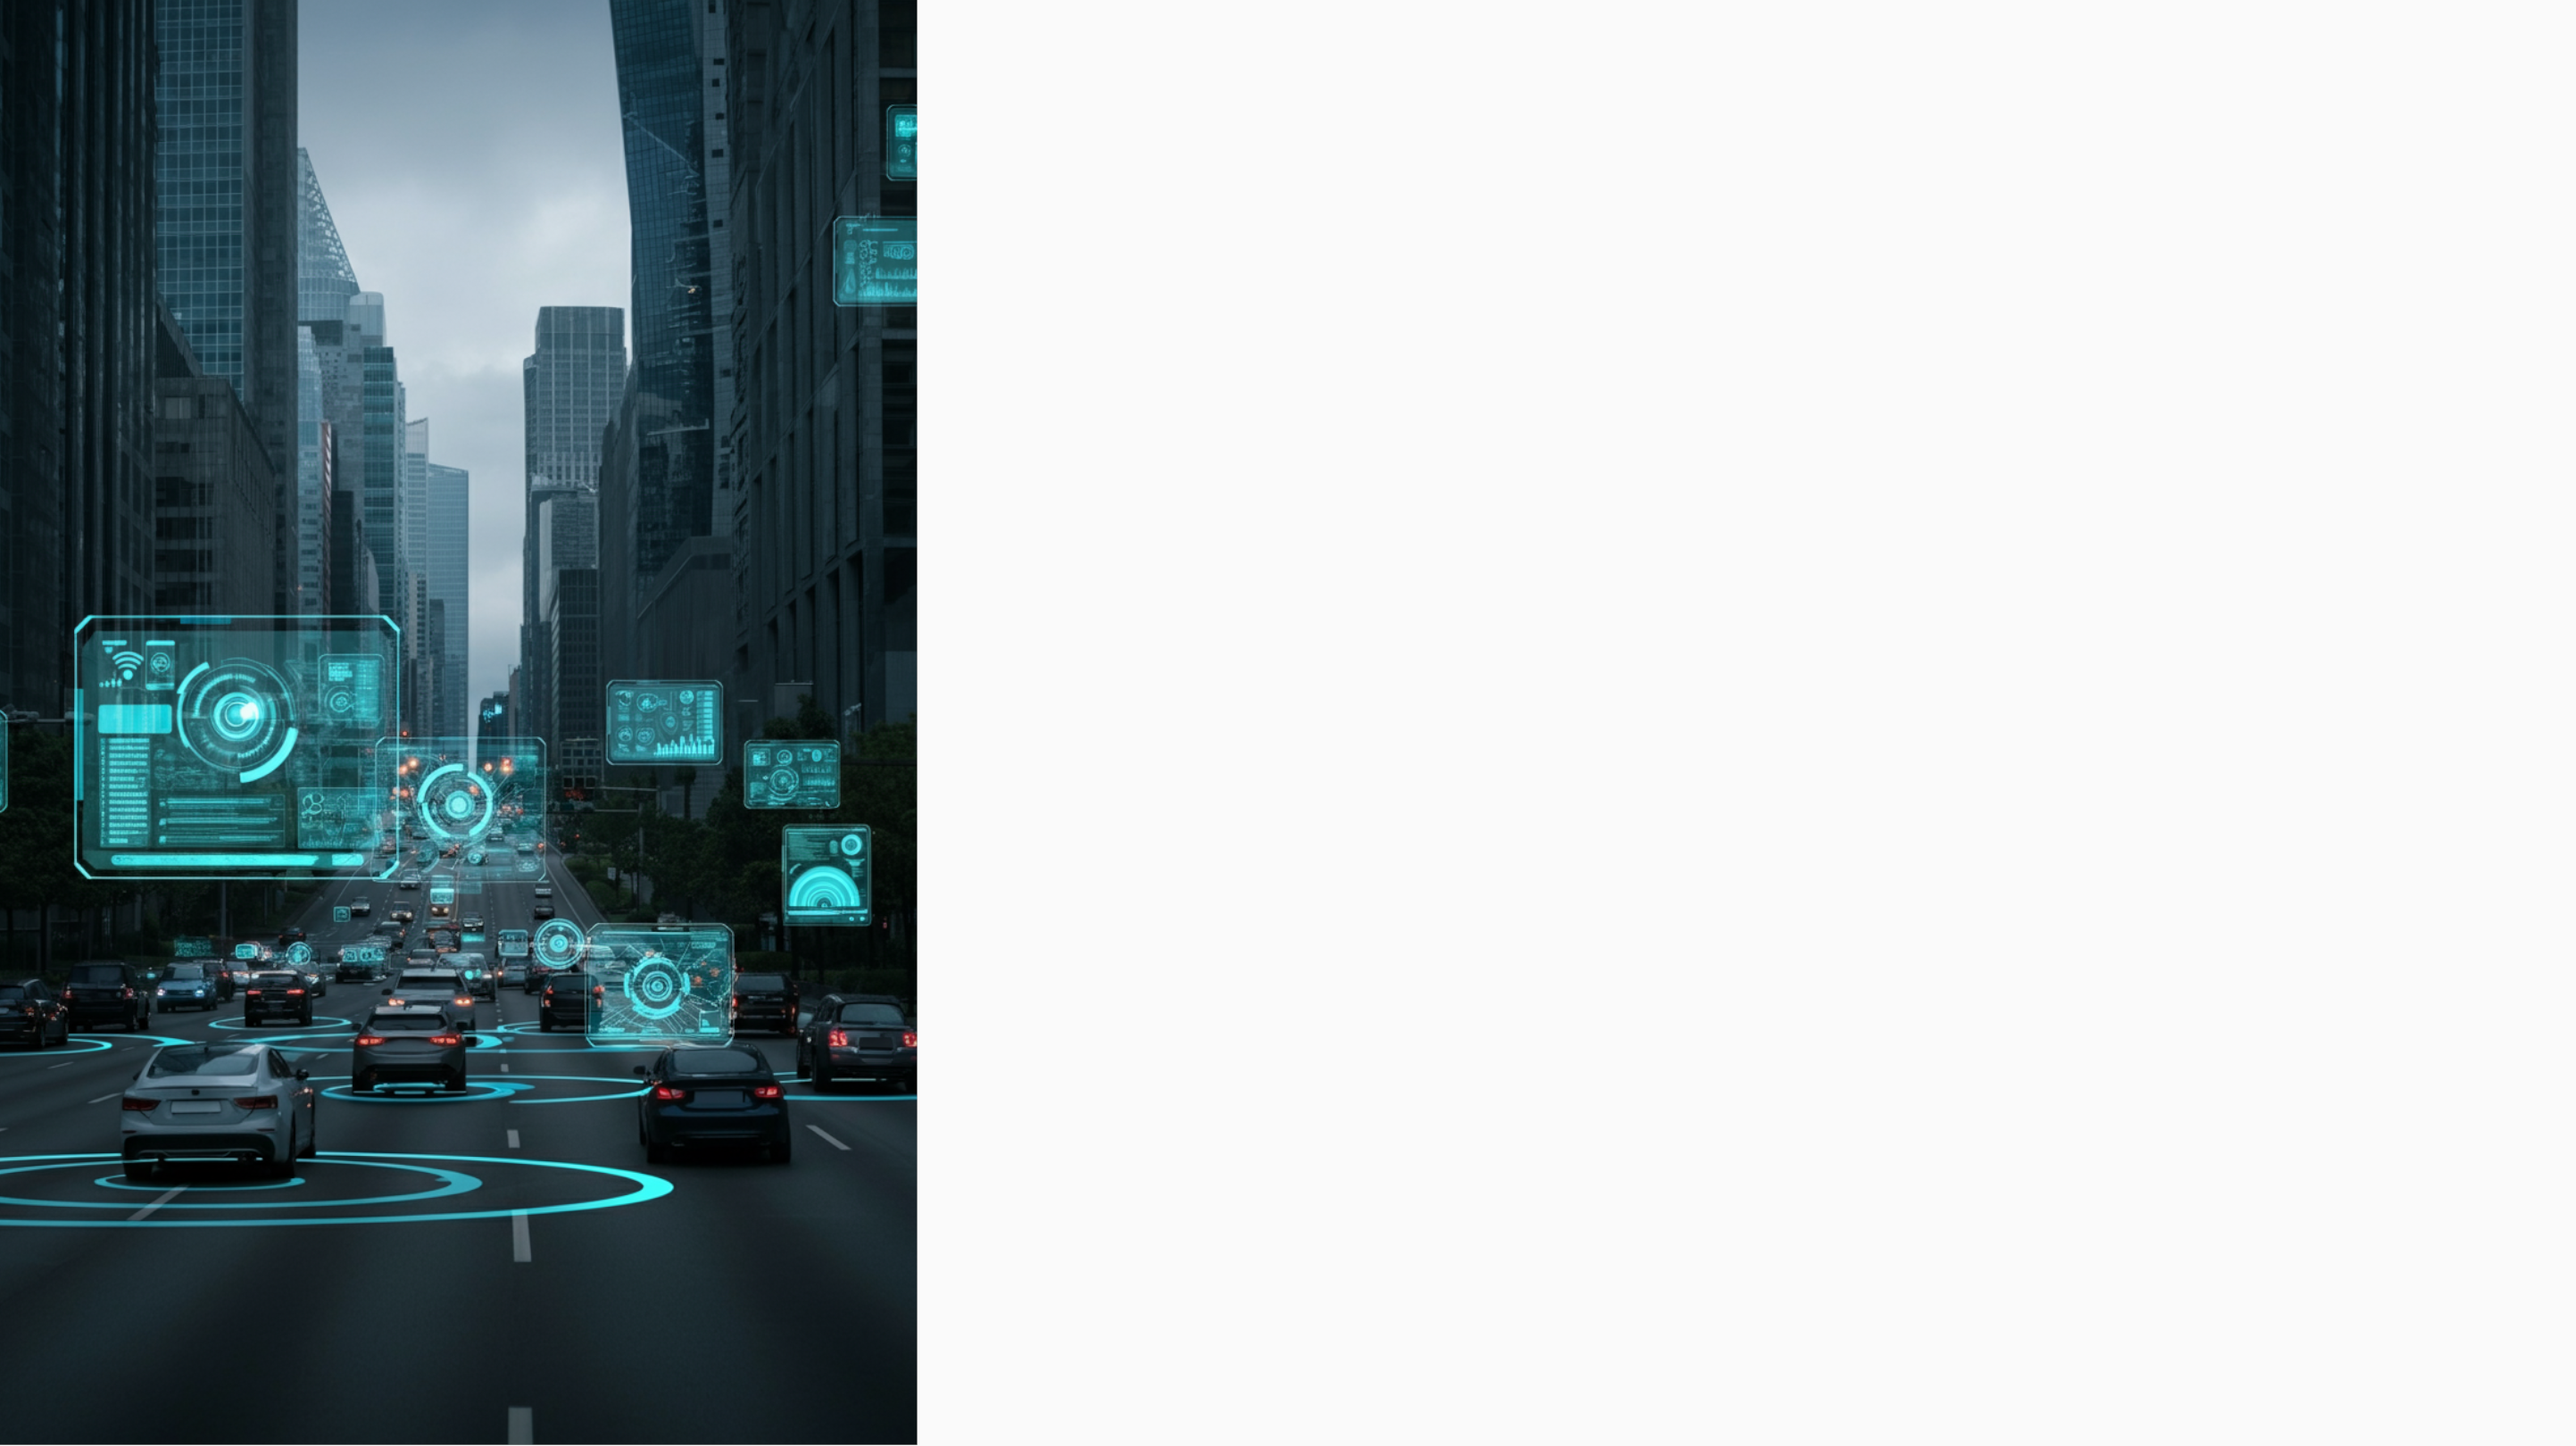
\includegraphics[width=\paperwidth,height=\paperheight]{img/frame-1.png}}
\begin{frame}\end{frame}
}
{
\usebackgroundtemplate%
{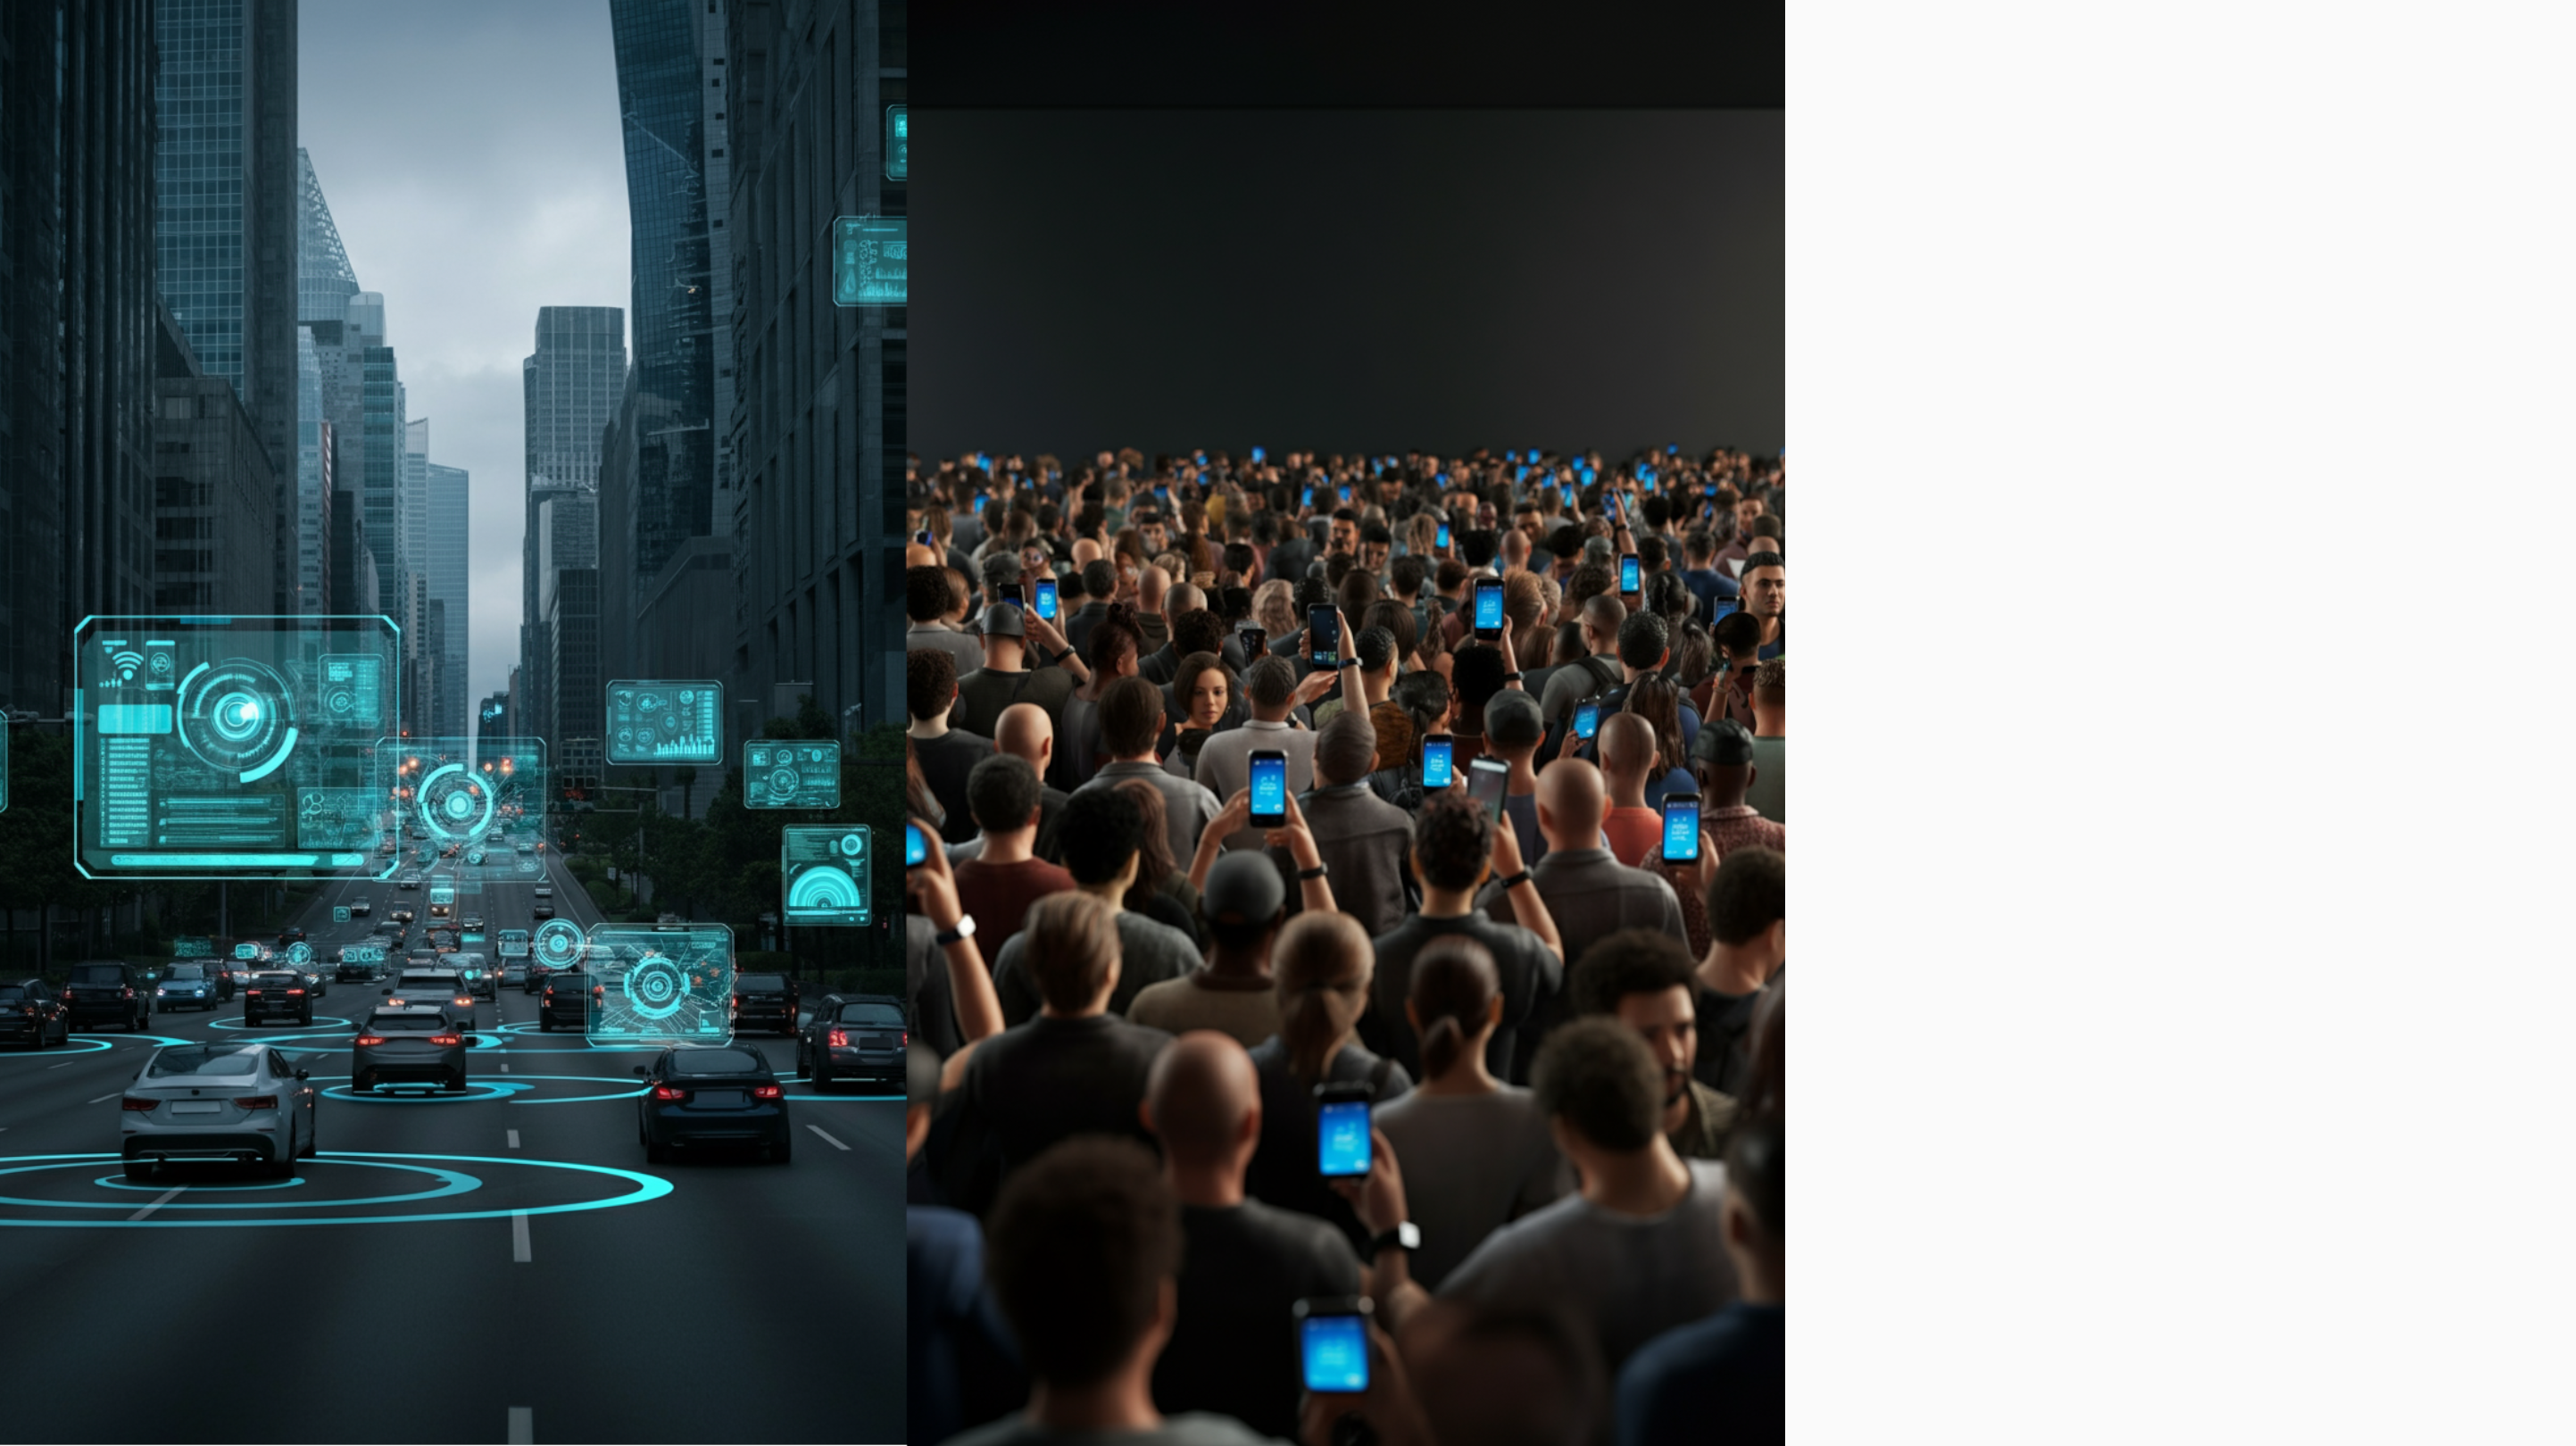
\includegraphics[width=\paperwidth,height=\paperheight]{img/frame-2.png}}
\begin{frame}\end{frame}
}
{
\usebackgroundtemplate%
{\includegraphics[width=\paperwidth,height=\paperheight]{img/frame-3.png}}
\begin{frame}\end{frame}
}
\begin{frame}{Panorama Computazionale Moderno}
	\begin{itemize}
		\item Centinaia/Migliaia di dispositivi computazionali
		\item Altamente eterogenei e distribuiti
		\item Interconnessi tramite reti di comunicazione
		\begin{itemize}
			\item \textbf{Internet of Things} (IoT)
		\end{itemize}
		\item Applicazioni \alert{\emph{situate}} e \alert{\emph{ubiquite}}
		\begin{itemize}
			\item Context-aware
			\item Pervasiveness (la computazione che ``scompare'')
		\end{itemize}
		\item L'umano è parte integrante del sistema
		\begin{itemize}
			\item Human-in-the-loop
		\end{itemize}
		\item \alert{\textbf{Come possiamo progettare sistemi artificiali che si adattano a questo contesto?}}
		\item \alert{\faLeaf} ~ Inspiriamoci a come la natura affronta problemi simili ~ \alert{\faLeaf}
	\end{itemize}
\end{frame}
\begin{frame}[fragile]{Animali Sociali}
% https://cric96.github.io/hello-aarhus/#/3/5/3
\begin{center}
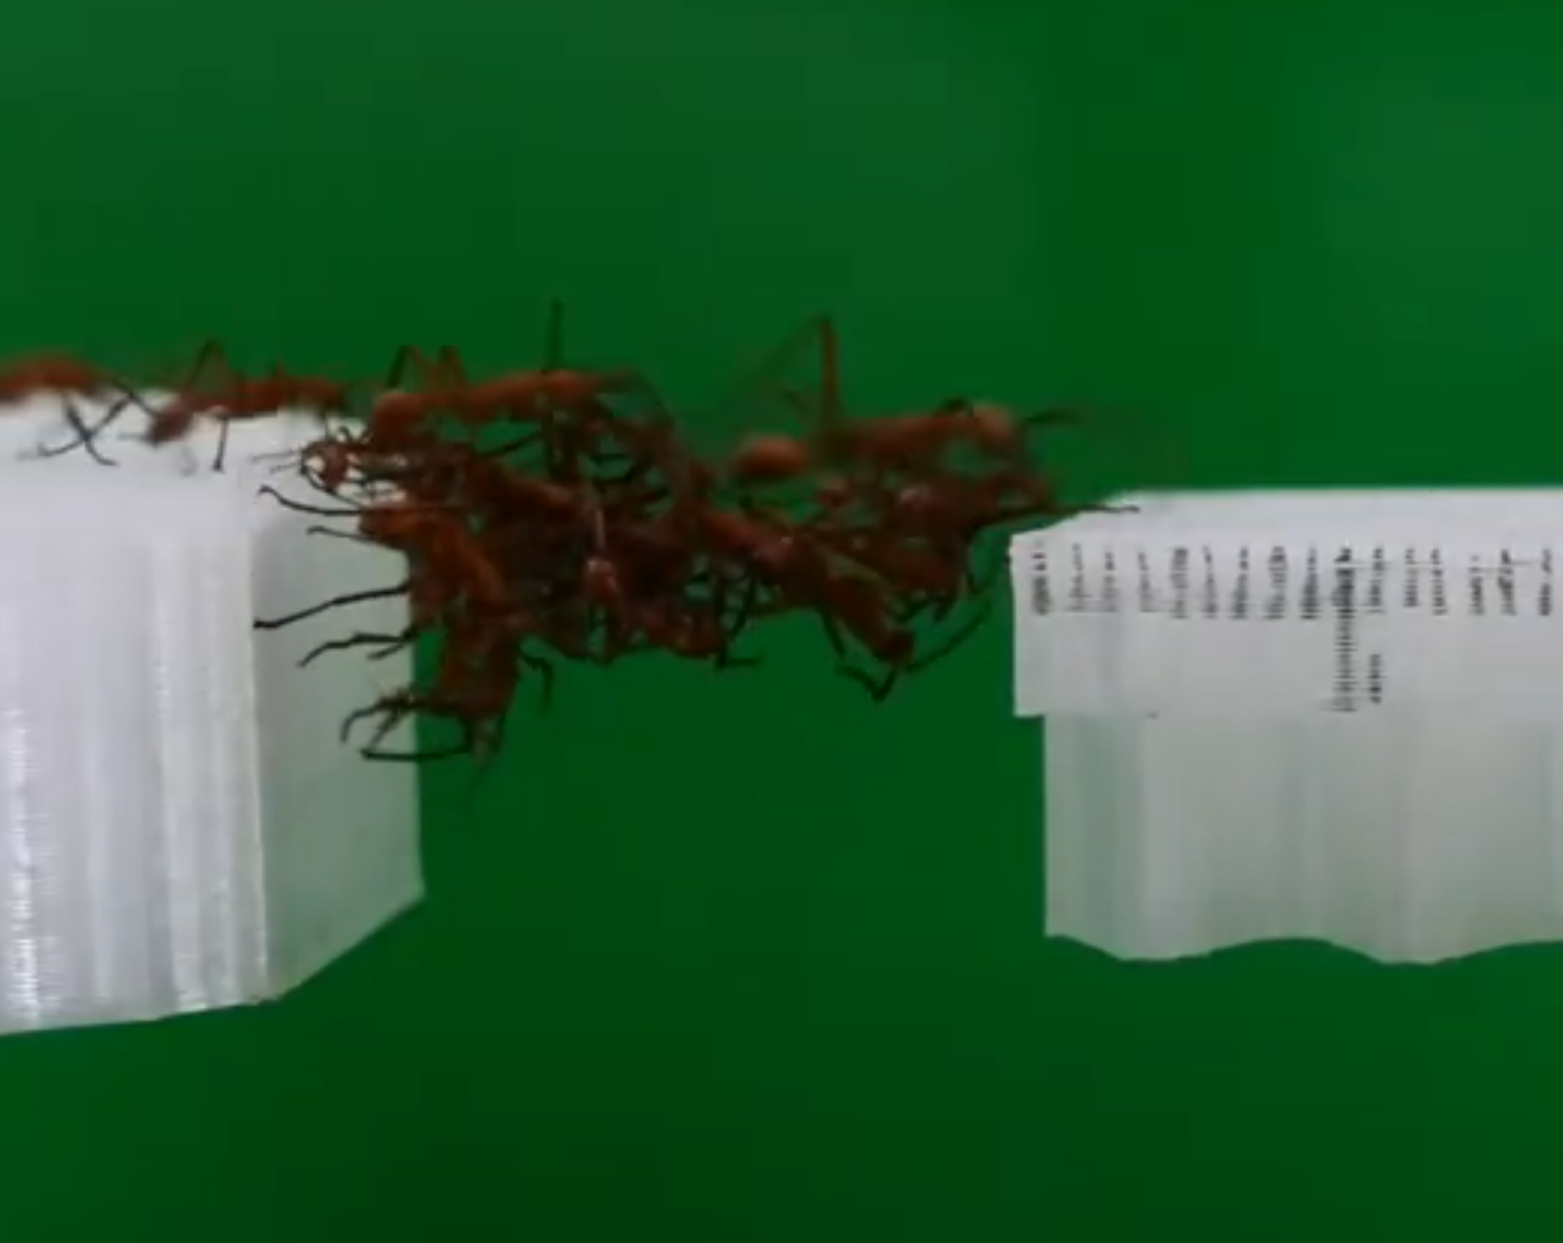
\includegraphics[height=3.7cm]{img/example.png}
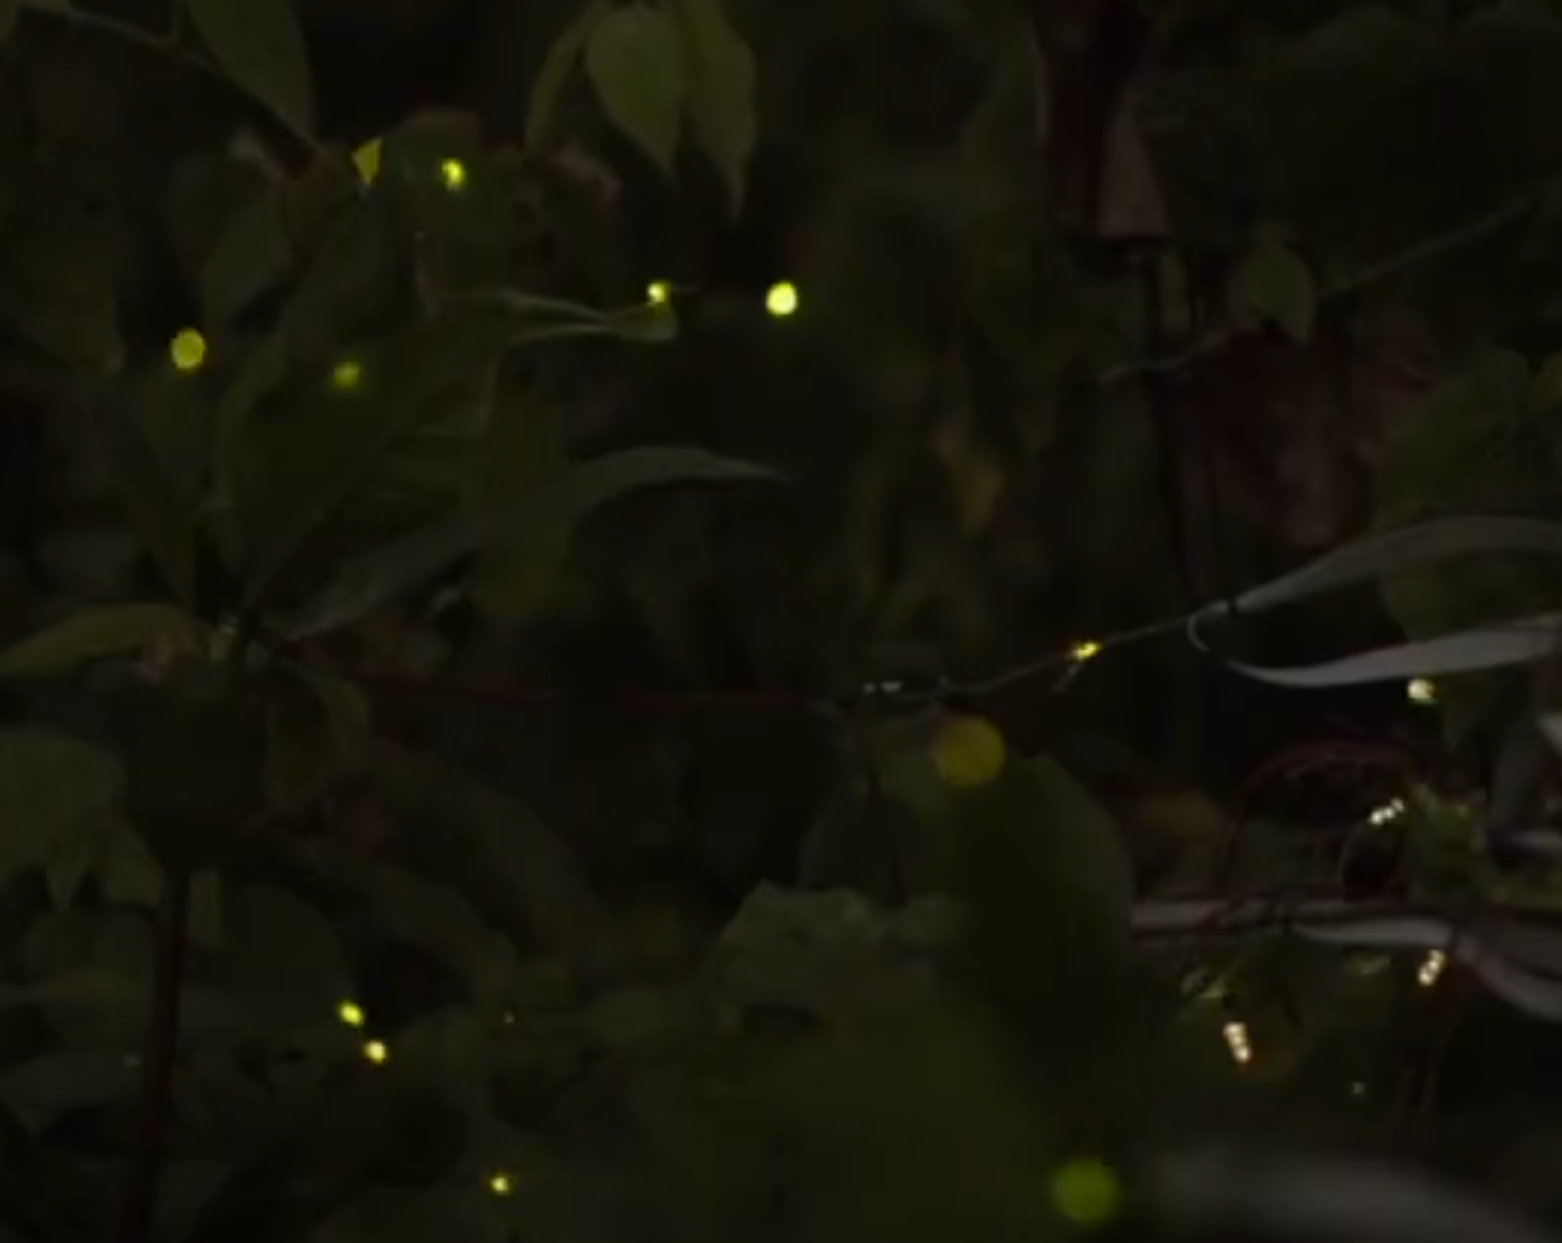
\includegraphics[height=3.7cm]{img/fireflies.png}
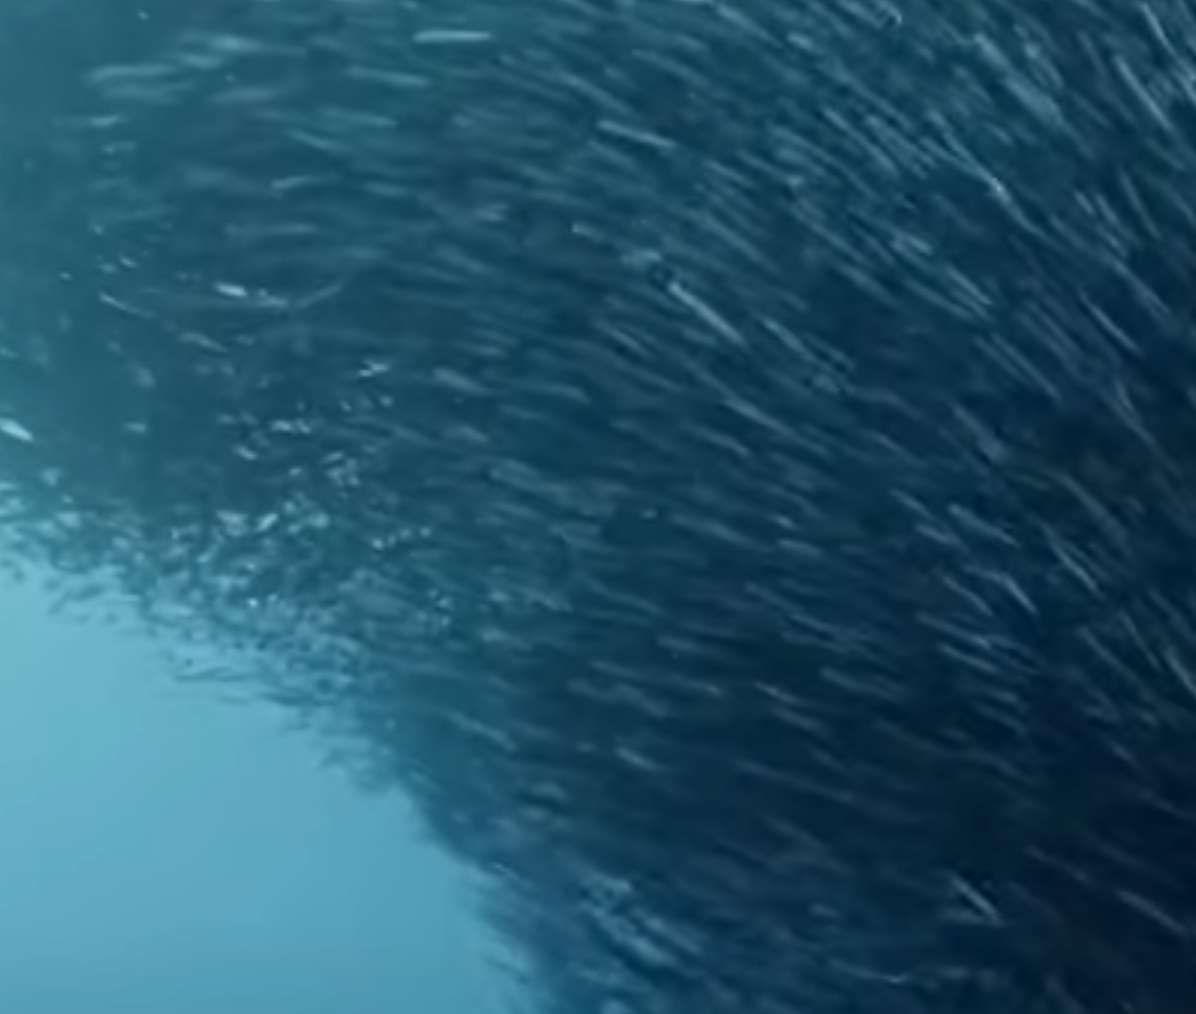
\includegraphics[height=3.7cm]{img/school.png}
\end{center}
In tutti questi scenari, gli animali/organismi mostrano una sorta di \underline{\alert{\textbf{intelligenza collettiva}}}.
\end{frame}
{

\setbeamercolor{background canvas}{bg=custombg} % Set background to foreground color
\setbeamercolor{normal text}{fg=customfg}    

\begin{frame}[c]
	
	{
	\color{customfg}

	\begin{center}
	\Large\textbf{Intelligenza Collettiva} \\
	
	L'\alert{\emph{intelligenza}} che può essere attribuita a un \alert{\emph{collettivo}}.
	\\ \vspace{1cm}
		\large{\alert{Intelligenza}} \faArrowRight ~ Misura la capacità di un agente di raggiungere \underline{\emph{obiettivi}} in un'ampia gamma di ambienti.  \\

		\large{\alert{Collettivo}} \faArrowRight ~ Gruppi di individui (membri) che manifestano una qualche forma di \underline{\emph{unità}}. \\
	\end{center}

	\vspace{1cm}	
}
\end{frame}
}
\begin{frame}{Intelligenza Collettiva E Sistemi Collettivi Adattativi}
	\begin{alertblock}{Definizioni -- Cont.}
		\begin{itemize}
			\item \emph{Gruppi di individui che agiscono collettivamente in modi che sembrano intelligenti.} -- focus sul concetto di \alert{gruppo}
			\item \emph{Intelligenza che emerge a livello macro di un collettivo e trascende quella dei singoli individui.} -- focus sul livello \alert{macro} e \alert{micro}
		\end{itemize}
	\end{alertblock}
	\begin{exampleblock}{Sottoclassi di Intellingenza Collettiva}
		\begin{itemize}
			\item Intellingenza di \emph{Sciame} (\alert{Swarm Intelligence}): Intelligenza collettiva osservata in gruppi di \emph{animali}
			\item Intelligenza di Folle (\alert{Crowd Intellingece}): Intelligenza collettiva osservata in gruppi di \emph {persone}
		\end{itemize}
	\end{exampleblock}
	\begin{block}{Sistemi Collettivi Adattativi (CAS)}
		Sistemi composti da un insieme di agenti autonomi che mostrano intellingenza collettiva.
	\end{block}
\end{frame}
\begin{frame}{Collective Adaptive System}
\begin{alertblock}{Caratteristiche (tratte dagli animali sociali)}
	\begin{itemize}
		\item \textbf{Decentralizzazione} \faArrowRight ~ Nessun controllo centrale
		\item \textbf{Adattabilità} \faArrowRight ~ Capacità di adattarsi a cambiamenti ambientali
		\item \textbf{Scalabilità} \faArrowRight ~ Capacità di crescere in numero di individui 
		\item \textbf{Emergenza} \faArrowRight ~ Comportamenti collettivi che emergono da interazioni locali
		\item \textbf{Robustezza} \faArrowRight ~ Capacità di sopportare guasti
	\end{itemize}	
\end{alertblock}

\begin{exampleblock}{Sfide ingegneristiche}
	\begin{itemize}
		\item \textbf{Fallimenti} \faArrowRight ~ I fallimenti del sistema (es. guasti, perdita dei messaggi, ecc.) sono così comuni che devono diventare parte del design
		\item \textbf{Mapping tra micro e macro} \faArrowRight ~ Come i comportamenti locali dei singoli agenti si traducono in comportamenti collettivi?
		\item \textbf{Unknown unknowns} \faArrowRight ~ Come progettare sistemi che si adattano a situazioni non previste?
	\end{itemize}
\end{exampleblock}
\end{frame}
\begin{frame}{Progettare Sistemi Collettivi Adattativi}
	\begin{itemize}
		\item \textbf{Approcci manuali} \faArrowRight ~ Programmazione inspirata (o basata su) sistemi biologici:
		\begin{itemize}
			\item \alert{Bottom-up} \faArrowRight ~ Si imita la natura per progettare sistemi collettivi adattativi
			\item \alert{Top-down} \faArrowRight ~ Inspirandosi dai meccanismi biologici, si introducuno nuove astrazioni per progettare sistemi collettivi adattativi
			\begin{itemize}
				\item \textbf{Macro programmazione} \faArrowRight ~ Linguaggi di programmazione che inseriscono il collettivo come entità di prima classe
			\end{itemize}
		\end{itemize}
		\item \textbf{Approcci automatici} \faArrowRight ~ Progettazione di sistemi collettivi adattativi tramite algoritmi automatici
		\begin{itemize}
			\item \alert{Algoritmi Genetici} \faArrowRight ~ Evoluzione di popolazioni di agenti
			\item \textbf{Apprendimento per Rinforzo Multi-Agente} \faArrowRight ~ Apprendimento per rinforzo in sistemi multi-agente
		\end{itemize}
	\end{itemize}

	È cruciale sfruttare le \alert{\textbf{simulazioni}} per testare le ipotesi e validare i modelli.
\end{frame}
\section{Approcci Manuali}


\subsection{Inspirati alla Biologia}

\begin{frame}{Soluzioni Swarm-inspired}
	\begin{exampleblock}{Definizione}
		Comportamenti collettivi emergono da interazioni locali tra agenti autonomi
	\end{exampleblock}
	\begin{block}{Come}
		\begin{itemize}
			\item \textbf{Comportamenti locali} \faArrowRight ~ Gli agenti seguono regole locali (inspirati dagli animali presi in considerazione)
			\item \textbf{Interazione} \faArrowRight ~ Gli agenti interagiscono tra loro e con l'ambiente
			\begin{itemize}
				\item Communicazione diretta 
				\item Indiretta (e.g., attraverso l'ambiente, stigmergia)
			\end{itemize}
			\item \textbf{Auto-organizzazione} \faArrowRight ~ Comportamenti collettivi emergono da interazioni locali
		\end{itemize}
	\end{block}
\end{frame}
\begin{frame}{Swarm-Inspired - Metropolitana di Tokyo}
	\centering
	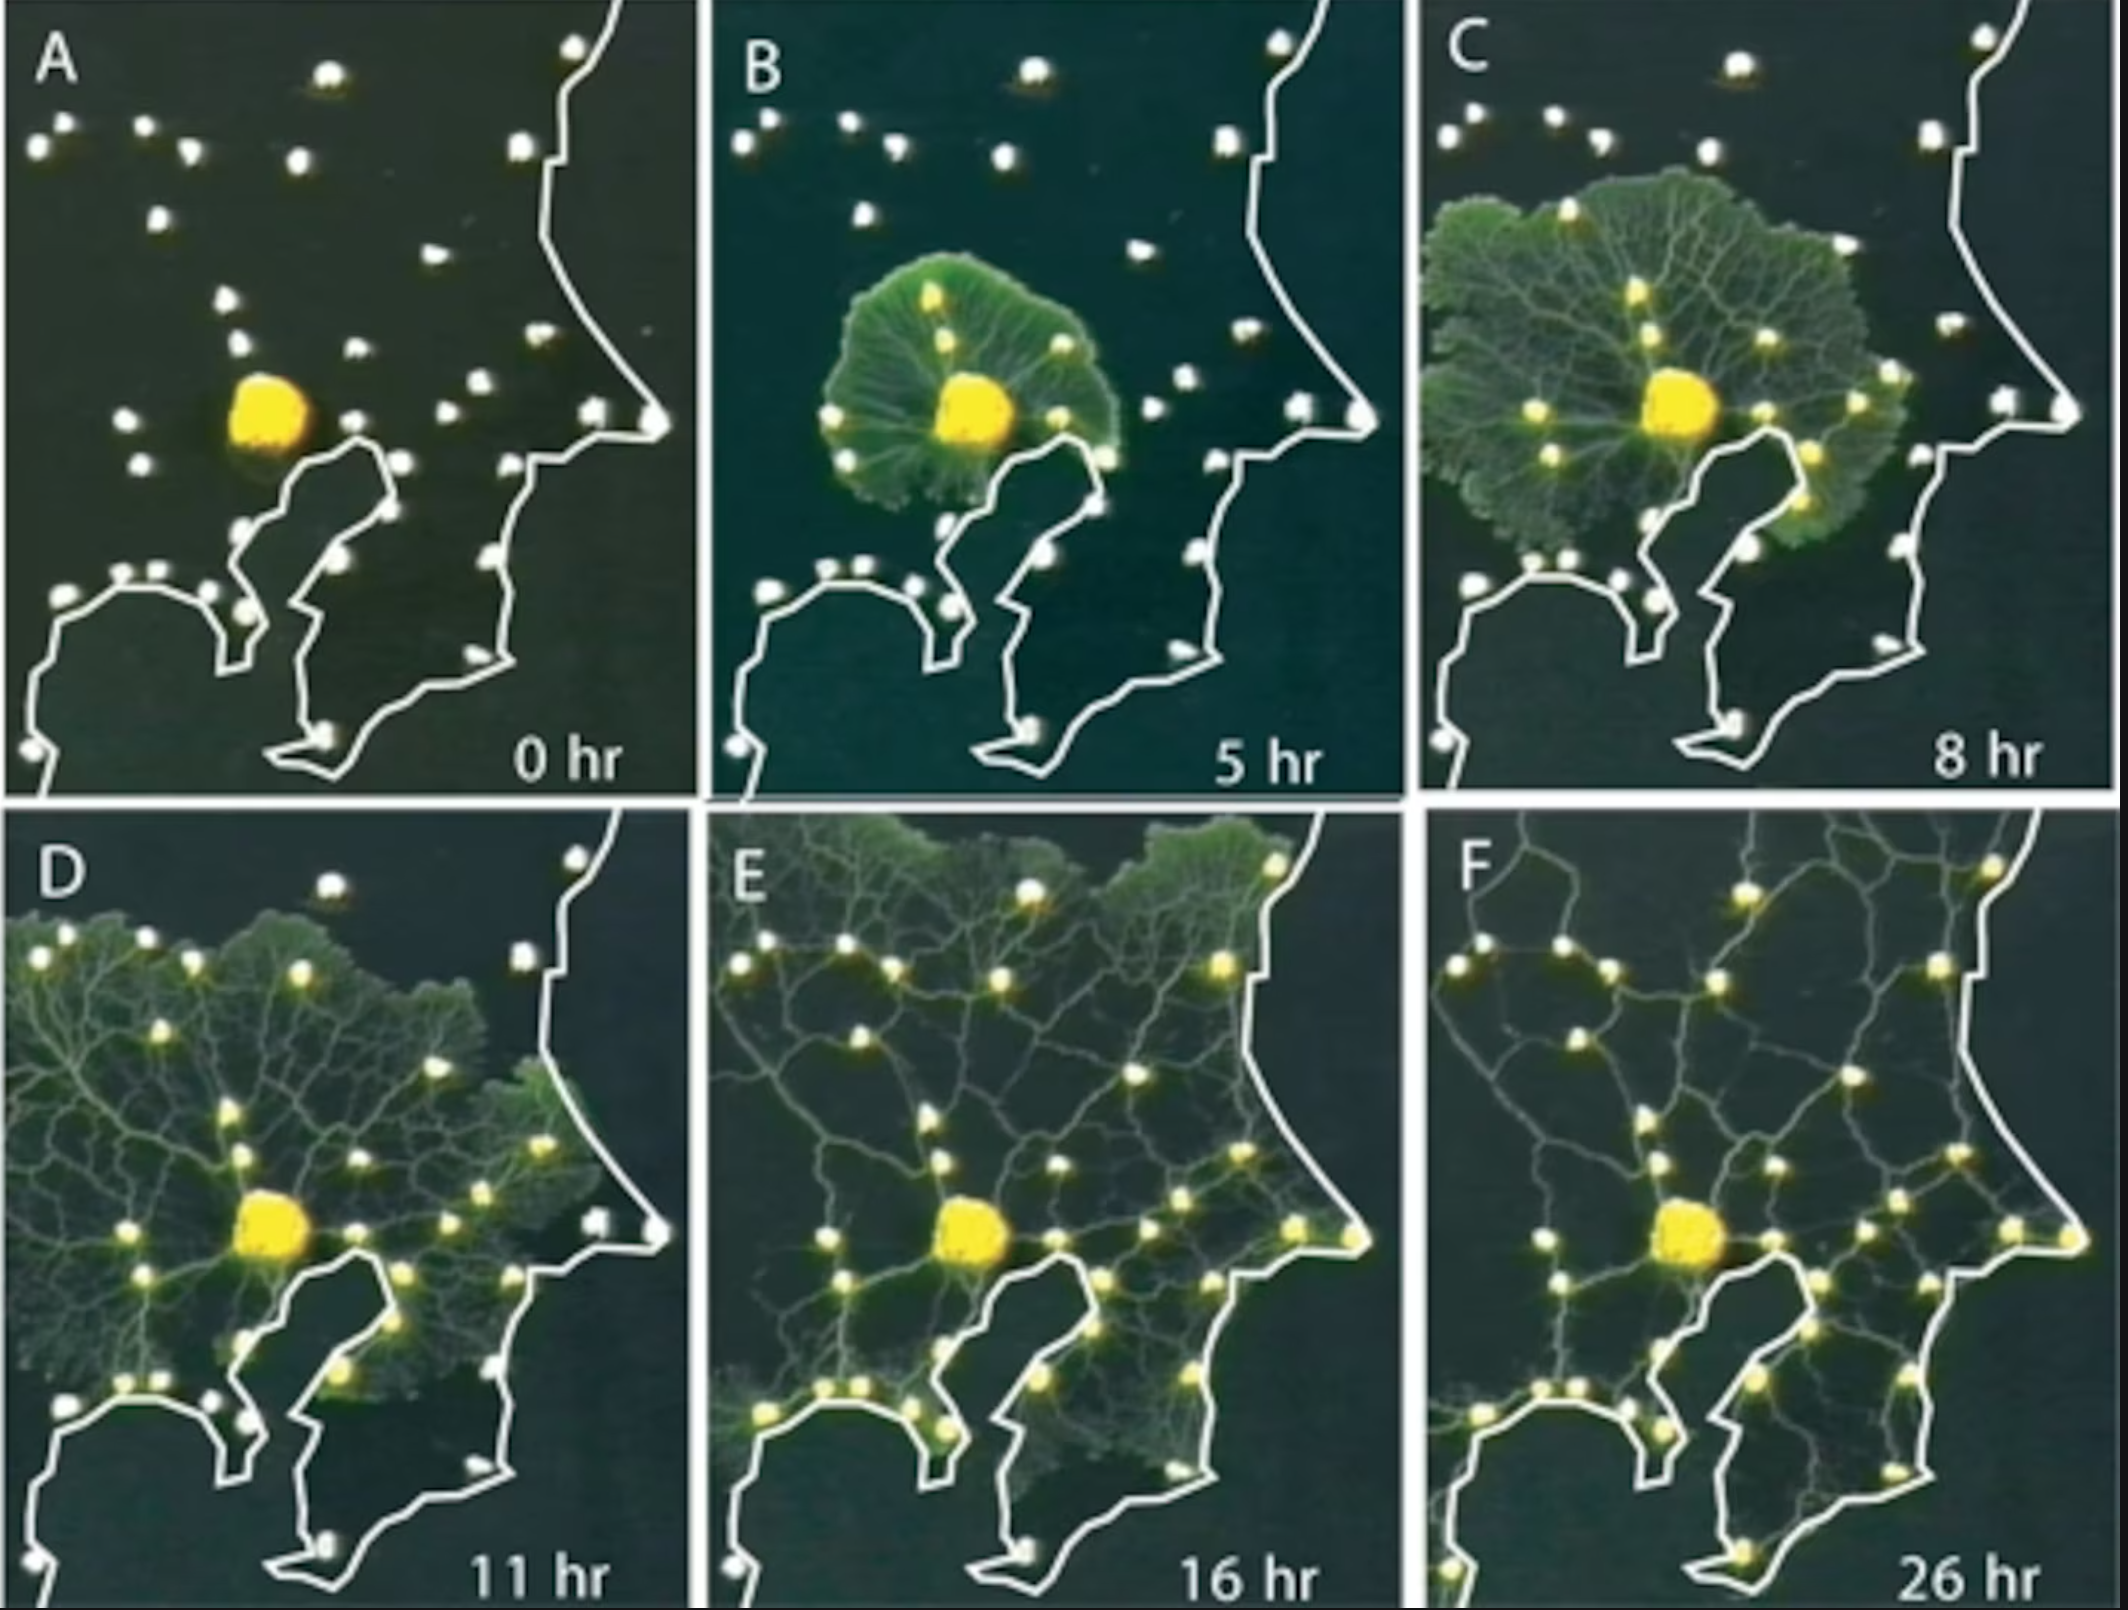
\includegraphics[width=0.6\textwidth]{img/metro-tokyo.png}
\end{frame}
\begin{frame}{Swarm-Inspired - Robotica di Sciame}
	\centering
	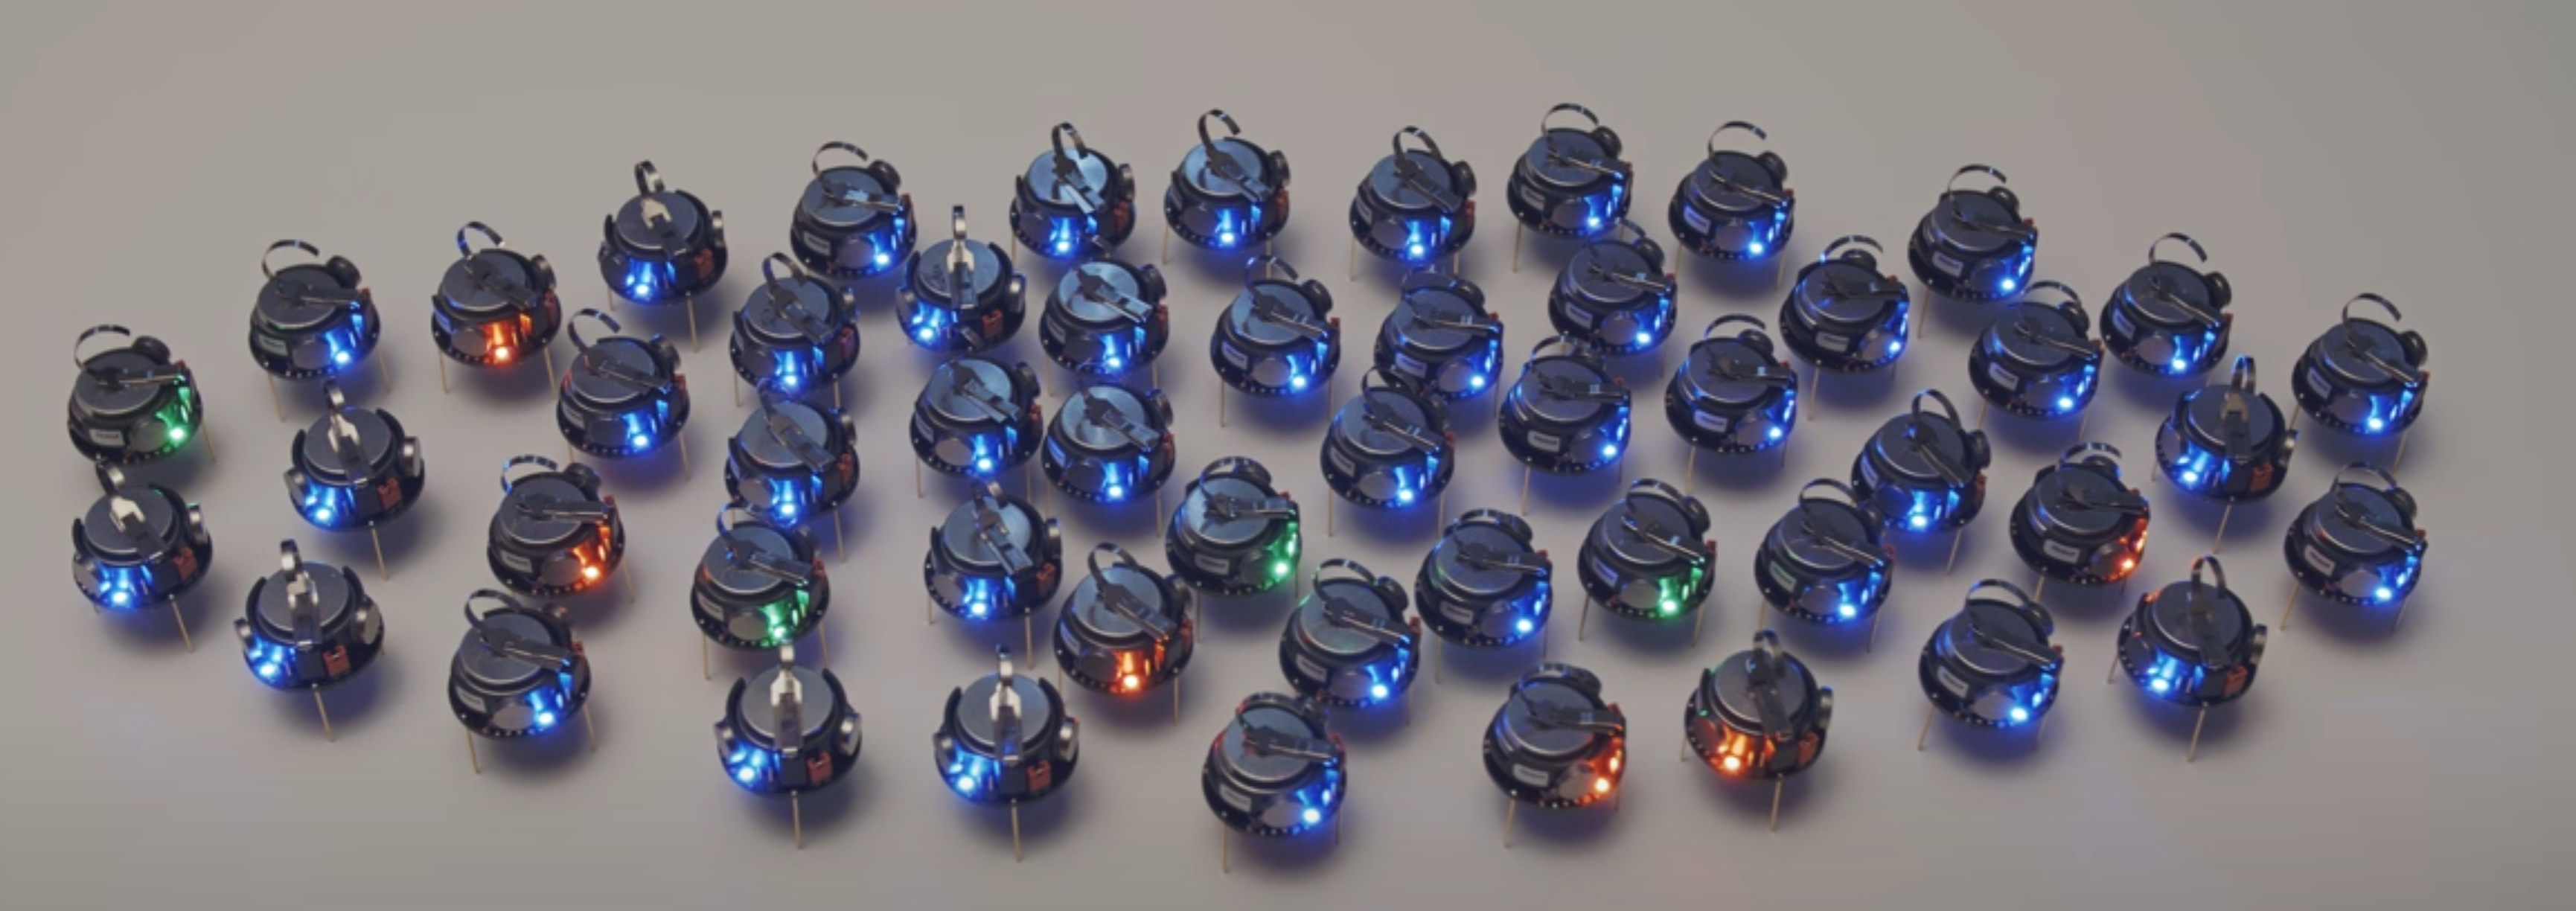
\includegraphics[width=\textwidth]{img/kilobot.png}
\end{frame}

\begin{frame}{Limiti degli algoritmi Swarm-Limiti degli algoritmi Swanspired}
\centering
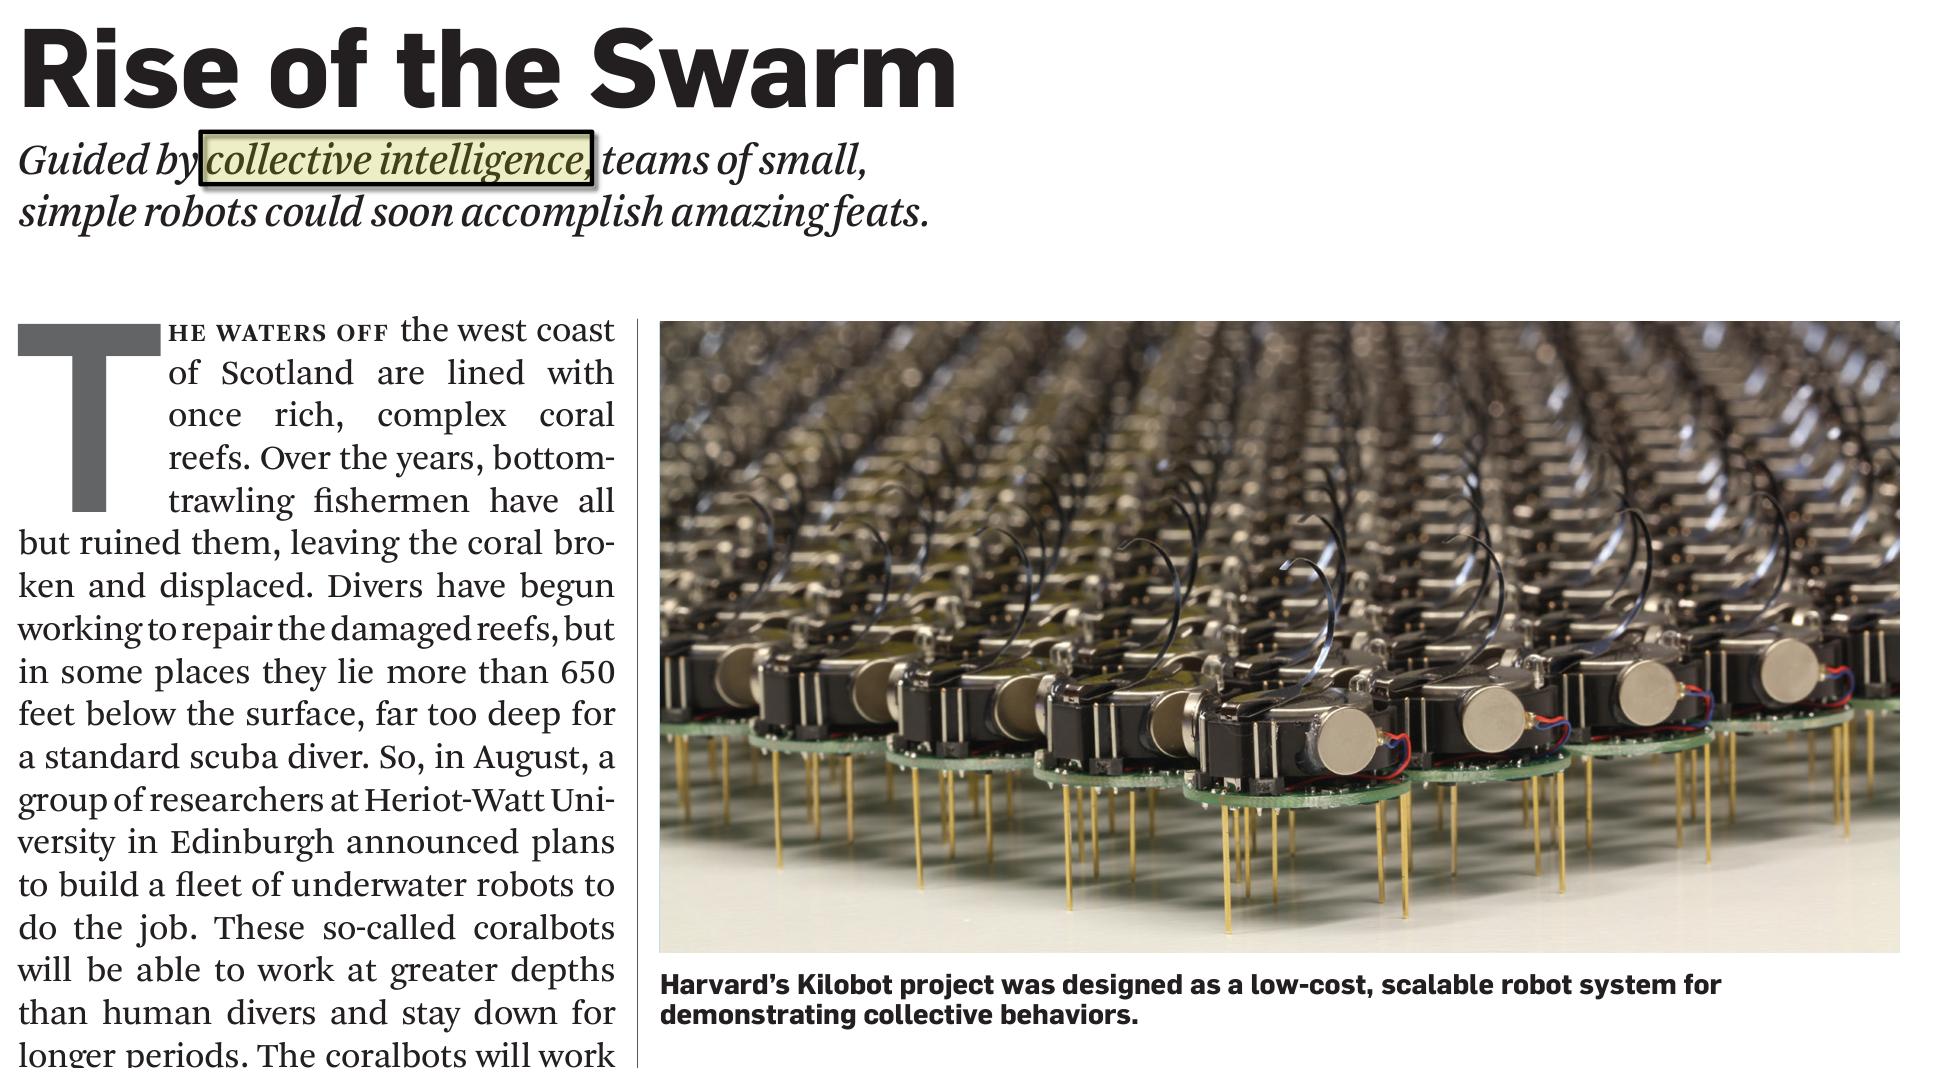
\includegraphics[width=0.8\textwidth]{img/rise-of-swarm.png}

{\color{red}\faThumbsDown}~\textbf{Abstraction Gap} {\color{red}\faThumbsDown} ~\textbf{Scalabilità} {\color{red}\faThumbsDown} ~\textbf{Robustezza} 
\end{frame}
%\begin{frame}{Limiti degli algoritmi Swarm-Inspired}
%	\begin{itemize}
%		\item \textbf{Abstraction Gap:} Progettare sistemi partendo da comportamenti locali è difficile visto che non è chiaro come questi si traducano in comportamenti collettivi
%		\item \textbf{Scalabilità:} Trovato un comportamento locale che funziona, è difficile combinarne più di uno in modo che il sistema collettivo funzioni (e.g.)
%		\item \textbf{Robustezza:} I sistemi basati su swarm intelligence sono spesso fragili e dipendi da parametri specifici
%	\end{itemize}
%\end{frame}

{

\setbeamercolor{background canvas}{bg=custombg} % Set background to foreground color
\setbeamercolor{normal text}{fg=customfg}    

\begin{frame}[c]
	
	{
	\color{customfg}

	\begin{center}
	\Large\textbf{Macro programmazione} \\
	Paradigmi di programmazione che trattano il \alert{collettivo} come \emph{entità di prima classe} (sotto qualche forma)
	\end{center}

	\vspace{1cm}	
}
\end{frame}
}
\begin{frame}{Macro programmazione}
	\begin{alertblock}{Perché}
		\begin{itemize}
			\item Carico cognitivo ridotto \faArrowRight ~ Si può pensare a livello di collettivo, non di singoli agenti (e.g. \emph{swarm programming})
			\item \emph{Abstraction gap} ridotto \faArrowRight ~ Si può progettare sistemi collettivi adattativi partendo da astrazioni più alte
			\item Risultati formali \faArrowRight ~ Si possono ottenere risultati formali su sistemi collettivi adattativi a partire dai linguaggi di programmazione
		\end{itemize}
	\end{alertblock}
	\begin{block}{Esempi}
		\begin{itemize}
			\item \textbf{Buzz}: Linguaggio di programmazione per sistemi swarm-based 
			\begin{itemize}
				\item Astrazione: \emph{swarm}
			\end{itemize}
			\item \alert{\textbf{Aggregate computing}}: Linguaggio di programmazione top-down per sistemi collettivi Adattativi
			\begin{itemize}
				\item Astrazione: \emph{campi computazionali}
			\end{itemize}
		\end{itemize}
	\end{block}
\end{frame}
\begin{frame}{Aggregate Computing - Intuizione}
	\centering
	\Large Programma l'\alert{aggregato}, non gli \emph{individui}
	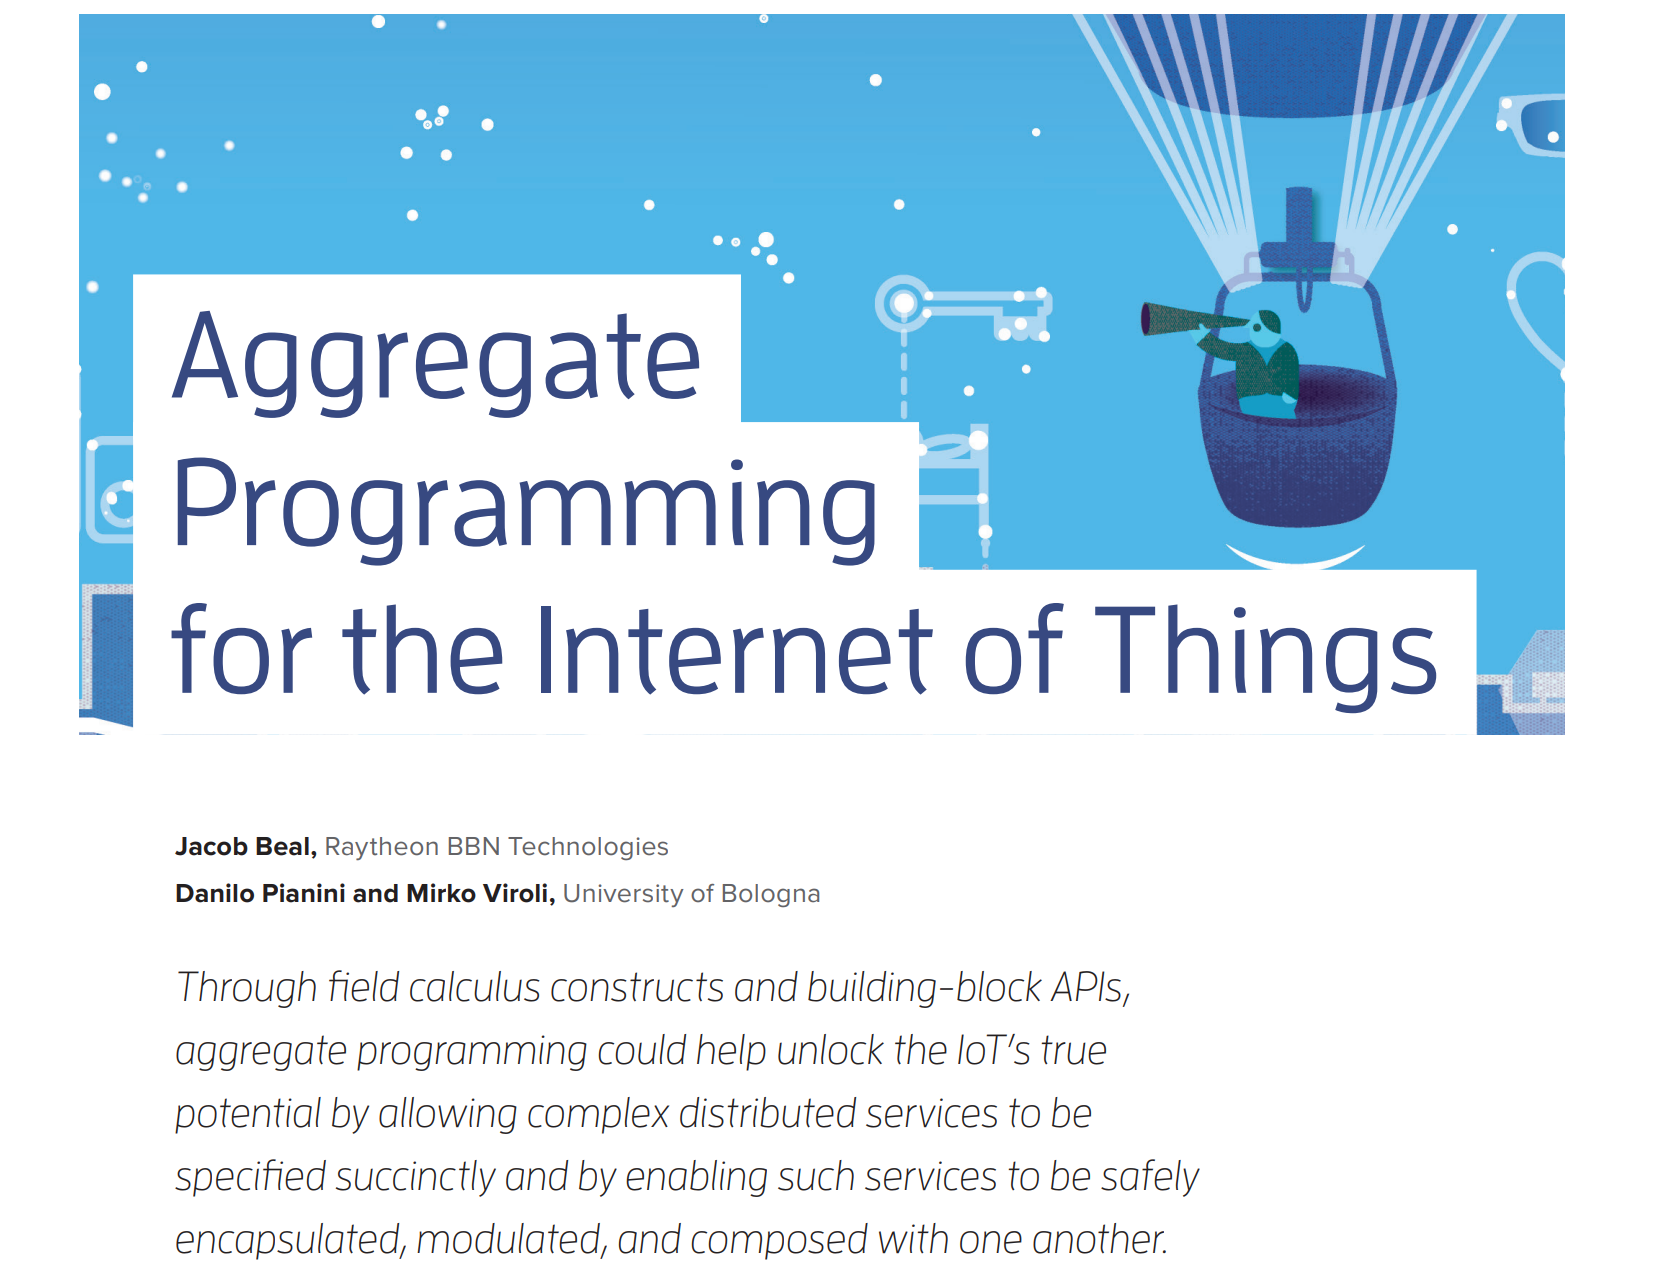
\includegraphics[width=0.6\textwidth]{img/overview.png}
\end{frame}
\begin{frame}{Aggregate Computing - Intuizione}
	\begin{center}
		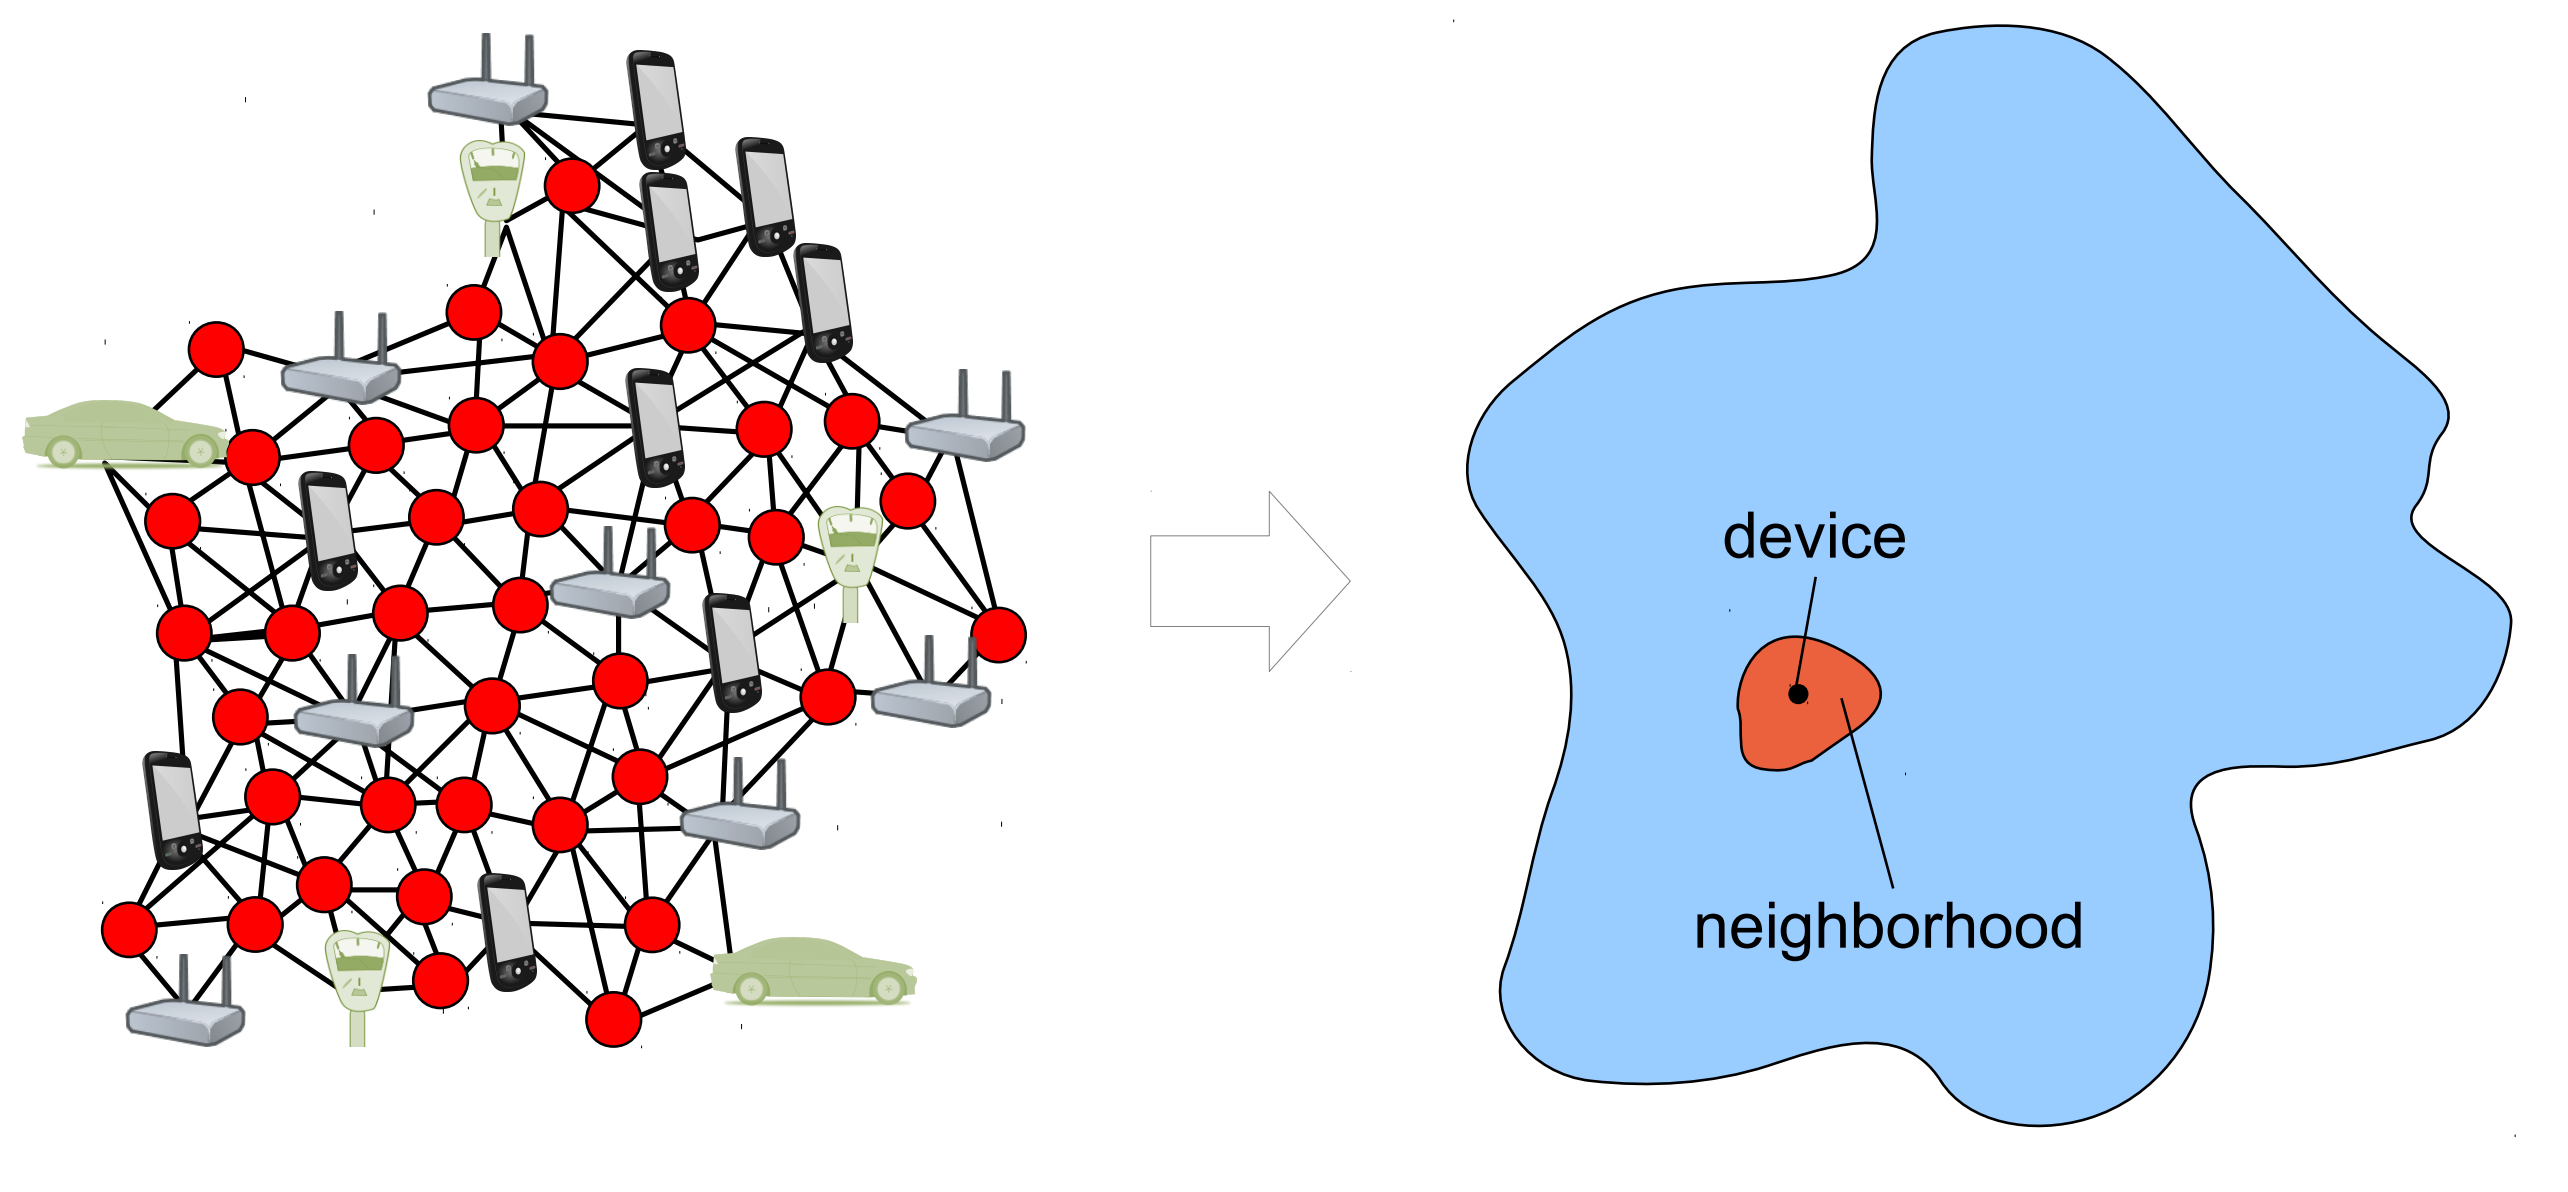
\includegraphics[width=0.4\textwidth]{img/ac.png}
		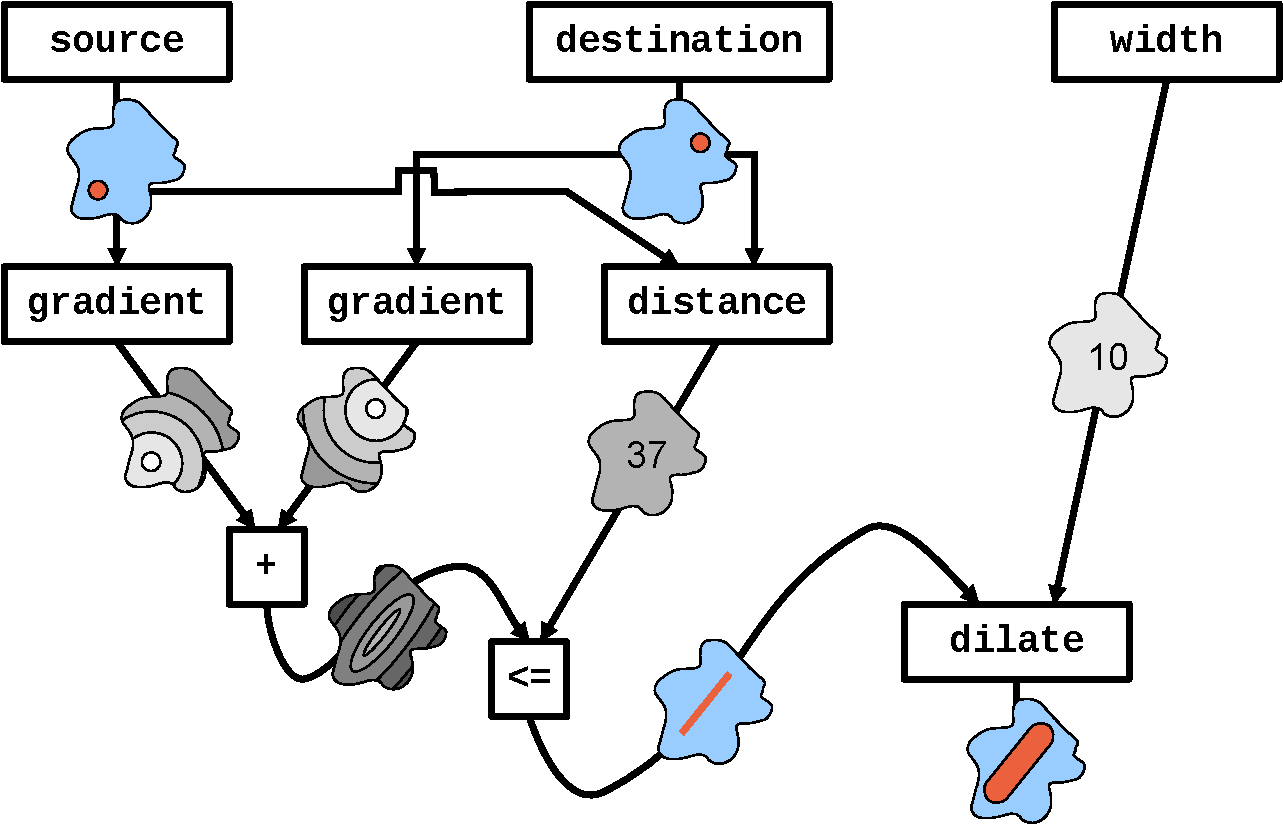
\includegraphics[width=0.4\textwidth]{img/channel.pdf}
	\end{center}
\end{frame}
\begin{frame}{Aggregate Computing - Casi di Studio}

\end{frame}
\begin{frame}{Aggregate Computing - Macro Swarm}

\end{frame}
\section{Approcci Automatici}
\begin{frame}{Limiti degli Approcci Manuali}
	\begin{itemize}
		\item \textbf{Adattabilità:} Progettare sistemi che si adattano a cambiamenti ambientali è difficile
		\begin{itemize}
			\item \emph{Unknown unknowns}
		\end{itemize}
		\item Come faccio a creare sistemi che si adattano all'ambiente senza doverli progettare manualmente?
		\begin{itemize}
			\item Osserviamo di nuova la natura :)
			\item Adattamento lento: \emph{evoluzione}
			\item Adattamento veloce: \emph{apprendimento}
		\end{itemize}
	\end{itemize}
\end{frame}
	\subsection{Algoritmi Genetici}
\begin{frame}{Algoritmi Genetici}

\end{frame}
\begin{frame}{Limiti degli Algoritmi Genetici}
\end{frame}
	\subsection{Apprendimento per Rinforzo multi-agente}

	{

	\setbeamercolor{background canvas}{bg=custombg} % Set background to foreground color
	\setbeamercolor{normal text}{fg=customfg}    
	
	\begin{frame}[c]
		
		{
		\color{customfg}
	
		\begin{center}
		\Large\textbf{Apprendimento Automatico} \\
		
		\end{center}
	
		\vspace{1cm}	
	}
\end{frame}
}
\begin{frame}{Modalità di Apprendimento}
	\begin{itemize}
		\item \textbf{Apprendimento Supervisionato} \faArrowRight ~ L'agente apprende da esempi etichettati
		\item \textbf{Apprendimento Non Supervisionato} \faArrowRight ~ L'agente apprende da esempi non etichettati
		\item \textbf{Apprendimento per Rinforzo} \faArrowRight ~ L'agente apprende da interazioni con l'ambiente
	\end{itemize}
\end{frame}
\begin{frame}{Apprendimento per Rinforzo}
	\begin{alertblock}{Definizione}
		\begin{itemize}
			\item \emph{Apprendimento per rinforzo} \faArrowRight ~ L'agente apprende a compiere azioni
		\end{itemize}
	\end{alertblock}
\end{frame}
\begin{frame}{Reti Neurali}
	\begin{itemize}
		\item \textbf{Perceptron} \faArrowRight ~ La più semplice rete neurale
		\item \textbf{Reti Neurali Convoluzionali} \faArrowRight ~ Usate per l'elaborazione di immagini
		\item \textbf{Reti Neurali Ricorrenti} \faArrowRight ~ Usate per l'elaborazione di sequenze
	\end{itemize}
\end{frame}
\begin{frame}{Apprendimento per Rinforzo Multi-Agente}

\end{frame}
\begin{frame}{Apprendimenti per Rinforzo Multi-Agente -- Esempi}

\end{frame}
\begin{frame}{Apprendimenti per Rinforzo Multi-Agente -- Assi}

\end{frame}
\section{Direzioni di Ricerca}
	\subsection{Sistemi Ibridi}
\begin{frame}{Sistemi Ibridi}

\end{frame}

\subsection{Modelli Fondazionali per l'Intelligenza Collettiva}
\begin{frame}{Modelli Fondazionali per l'Intelligenza Collettiva}

\end{frame}
\begin{frame}{Takeaways}
	\begin{itemize}
		\item \textbf{Intelligenza Collettiva} \faArrowRight ~ Intelligenza che emerge da gruppi di individui
		\item \textbf{Sistemi Collettivi Adattativi} \faArrowRight ~ Sistemi composti da agenti autonomi che mostrano intelligenza collettiva
		\item Progettazione di sistemi collettivi adattativi
		\begin{itemize}
			\item \emph{Approcci manuali} \faArrowRight ~ Programmazione ispirata alla biologia, macro programmazione
			\item \emph{Approcci automatici} \faArrowRight ~ Algoritmi genetici, apprendimento per rinforzo multi-agente
		\end{itemize}
		\item Direzioni di ricerca
		\begin{itemize}
			\item \emph{Sistemi ibridi}
			\begin{itemize}
				\item \emph{Approcci automatici} + \emph{Approcci manuali}
			\end{itemize}
			\item \emph{Modelli fondazionali}
			\begin{itemize}
				\item Insieme di reti neurali che catturano l'intelligenza collettiva
			\end{itemize}
		\end{itemize}
	\end{itemize}
\end{frame}
%//
%===============================================================================

%/////////

%===============================================================================
\section*{\refname}
%===============================================================================

%/////////

%%%%%%%%%%%%%%%%%%%%%%%%%%%%%%%%%%%%%%%%%%%%%%%%%%%%%%%%%%%%%%%%%%%%%%%%%%%%%%%%
\end{document}
%%%%%%%%%%%%%%%%%%%%%%%%%%%%%%%%%%%%%%%%%%%%%%%%%%%%%%%%%%%%%%%%%%%%%%%%%%%%%%%%
